\documentclass[12pt]{article}
\usepackage{amsmath}
\usepackage{setspace}

% for using images
\usepackage[pdftex]{graphicx}

% for caption manipulation
\usepackage{ccaption}

% Change the format of a figure caption
\captionnamefont{\bfseries}
\captiontitlefont{\small\sffamily}
\captiondelim{ --- }
\hangcaption
\renewcommand{\figurename}{Figure.}

% bibliography packages
\usepackage[sort&compress]{achemso}
%\citestyle{achemso}

\usepackage{fullpage}
\begin{document}

% some formatting tags
%\oddsidemargin  0.0in
%\evensidemargin 0.0in
%\textwidth      7.5in

% for angstrom symbols
\newcommand{\ang}{\,$\textrm{\AA}$}
\newcommand{\angs}{\ang}
\newcommand{\wat}{H$_2$O}
\newcommand{\ctc}{CCl$_4$}
\newcommand{\ctcwat}{CCl$_4$-H$_2$O}
\newcommand{\airwat}{air-H$_2$O}
\newcommand{\cl}{Cl$^-$}
\newcommand{\nit}{${\text{NO}_3}^-$}
\newcommand{\sul}{${\text{SO}_4}^{2-}$}
\newcommand{\nacl}{NaCl}
\newcommand{\sodnit}{NaNO$_3$}
\newcommand{\sodsul}{Na$_2$SO$_4$}
\newcommand{\costheta}{$\cos\theta$~}
\newcommand{\cosphi}{$\cos\phi$~}
\newcommand{\costhetarange}{~$<\cos\theta<$~}
\newcommand{\cosphirange}{~$<\cos\phi<$~}
\newcommand{\cm}{\,$cm^{-1}$}

\doublespacing

\section {Supporting Information}

Included here are the results of supplementary calculations regarding the electric field and the $\chi^{(2)}$ spectra from the molecular dynamics simulations.

\subsection {Electric Field}

The ``field-screening'' effect of the various ions in the solution can be quantified from the experimental and calculated SFG spectra. However, to verify that the location of the ions in the solution and the interface do affect the field as predicted, calculations were performed to determine the electric field throughout the interface. The classical formula for the electric field due to a point charge in space is given below in Equation \ref{classical_efield}

\begin{equation}\label{classical_efield}
	\bar{E}=\frac{1}{4\pi\epsilon_0}\frac{q}{r^2}\hat{\mathbf{r}}
\end{equation}

Whereas the $x$ and $y$ components of the electric field are assumed to be isotropic because of the system symmetry within the plane of the interface, the $z$ component can reduce to Equation \ref{z_efield}

\begin{equation}\label{z_efield}
	E_z \propto \frac{q}{r_z^2}
\end{equation}

One measure of the electric field normal to the interfacial plane, $E_z$, is thus accomplished by iterating over all point charge (atoms) contributions within the system. The electric field contributions as calculated from Equation \ref{z_efield} were summed and averaged over all the simulation configurations to produce the electric field response as shown in Figure \ref{fig:e_field} below.

\begin{figure}[h!]
\begin{center}
	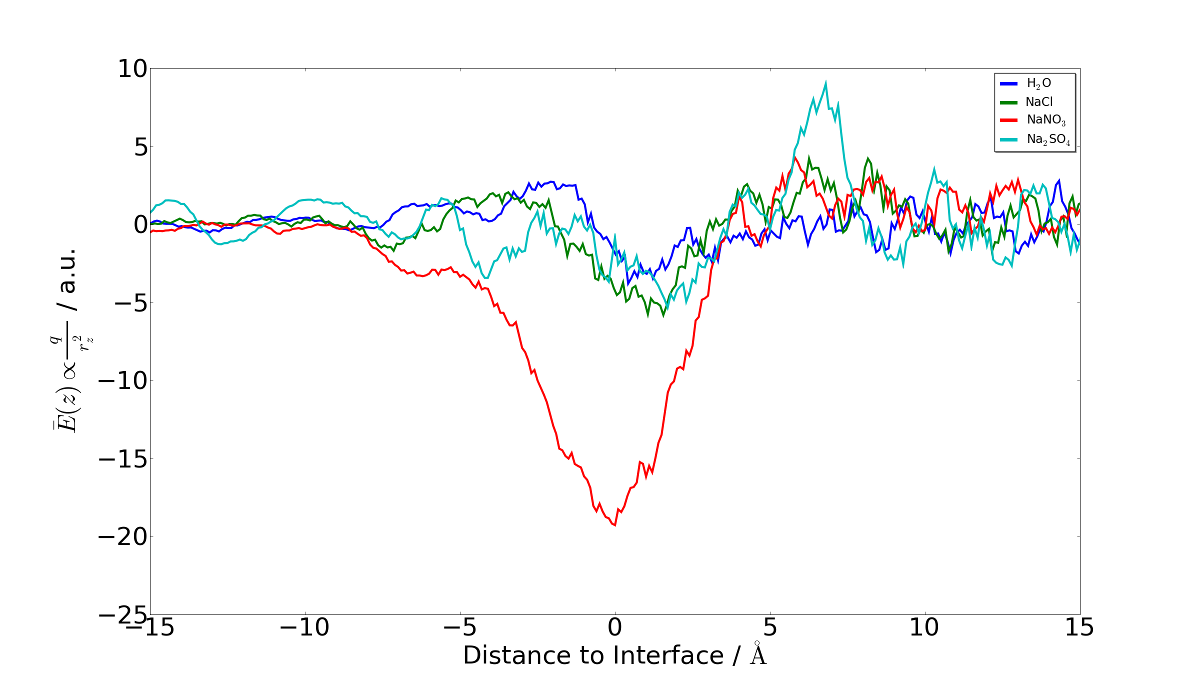
\includegraphics[scale=1.0]{images/electricfield.png}
	\caption{Interfacial net electric field. The field, as calculated by Equation \ref{z_efield}, varies across the interface for the different aqueous salt systems. Distances to the interface are positive on the aqueous salt side, and negative in the CCl$_4$ phase.}
	\label{fig:e_field}
\end{center}
\end{figure}

The E-field plots of the three salt systems vary from the pure \ctcwat~plot. The \nacl~system most closely matches the features of the \ctcwat~E-field. The \sodnit~system introduces a large negative feature centered about the GDS location where the \nit~anions are most accumulated. \sodsul~appears to match the \ctcwat~system features closely until the large positive peak at 7.0\angs~into the water phase - the approximate location of the sodium cation density enhancement.

Ion layering in the three salt systems exhibit specific trends that lead to these field intensities. The \nacl~ion density enhancements are broad, and the ions are located closely together such that the E-field is essentially cancelled by the counter-ions close to the double-layer, and dimishes quickly outside of a narrow region as a function of $\frac{1}{r^2}$. The \sodsul~system also exhibits a narrow ion double-layer within the aqueous phase, with the cation peak broader than the anion. This results in the slightly more positive field within the aqueous phase. The \sodnit~system exhibits two relatively widely spaced counter-ions with a broad cation density enhancement in the aqueous phase, and a pronounced anion enhancement near the GDS in the organic phase. This results in the very strong negative field around the GDS.

The closely-matched fields of the \ctcwat~and the \nacl~interfaces suggest that the resulting field felt by the interfacial waters will be similar. Thus the SFG spectra are not altered greatly between the two systems. The large negative field dominating the topmost interface region in the \sodnit~system affects the waters furthest out from the bulk water phase. This does not affect the deeper and more highly-coordinated waters as greatly as if the field enhancement were shifted further into the water bulk. Thus the deeper waters giving rise to the lower frequency OH-vibrational features are not as oriented or affected as the those closer to the GDS. Additionally, because the interface of the \sodnit~system is the narrowest of the systems, there are fewer waters affected at the surface than in the other aqueous salt solutions. Thus the ``free-OH'' SFG signal remains unchanged. The \sodsul~salt system exhibits the slightly larger positive field deep approx. 7\angs~within the solution. The field near the GDS is similar to the neat-\ctcwat~system and does not greatly affect the ``free-OH'' oscillators. However, the deeper field enhancement orients the more coordinated waters giving rise to the lower frequency SFG signal, as seen in the calculated SFG spectra.

\subsection{$\chi^{(2)}$}

Provided below are the real and imaginary components of the calculated $\chi^{(2)}$ spectra presented in the main work.

\begin{figure}[h!]
\begin{center}
	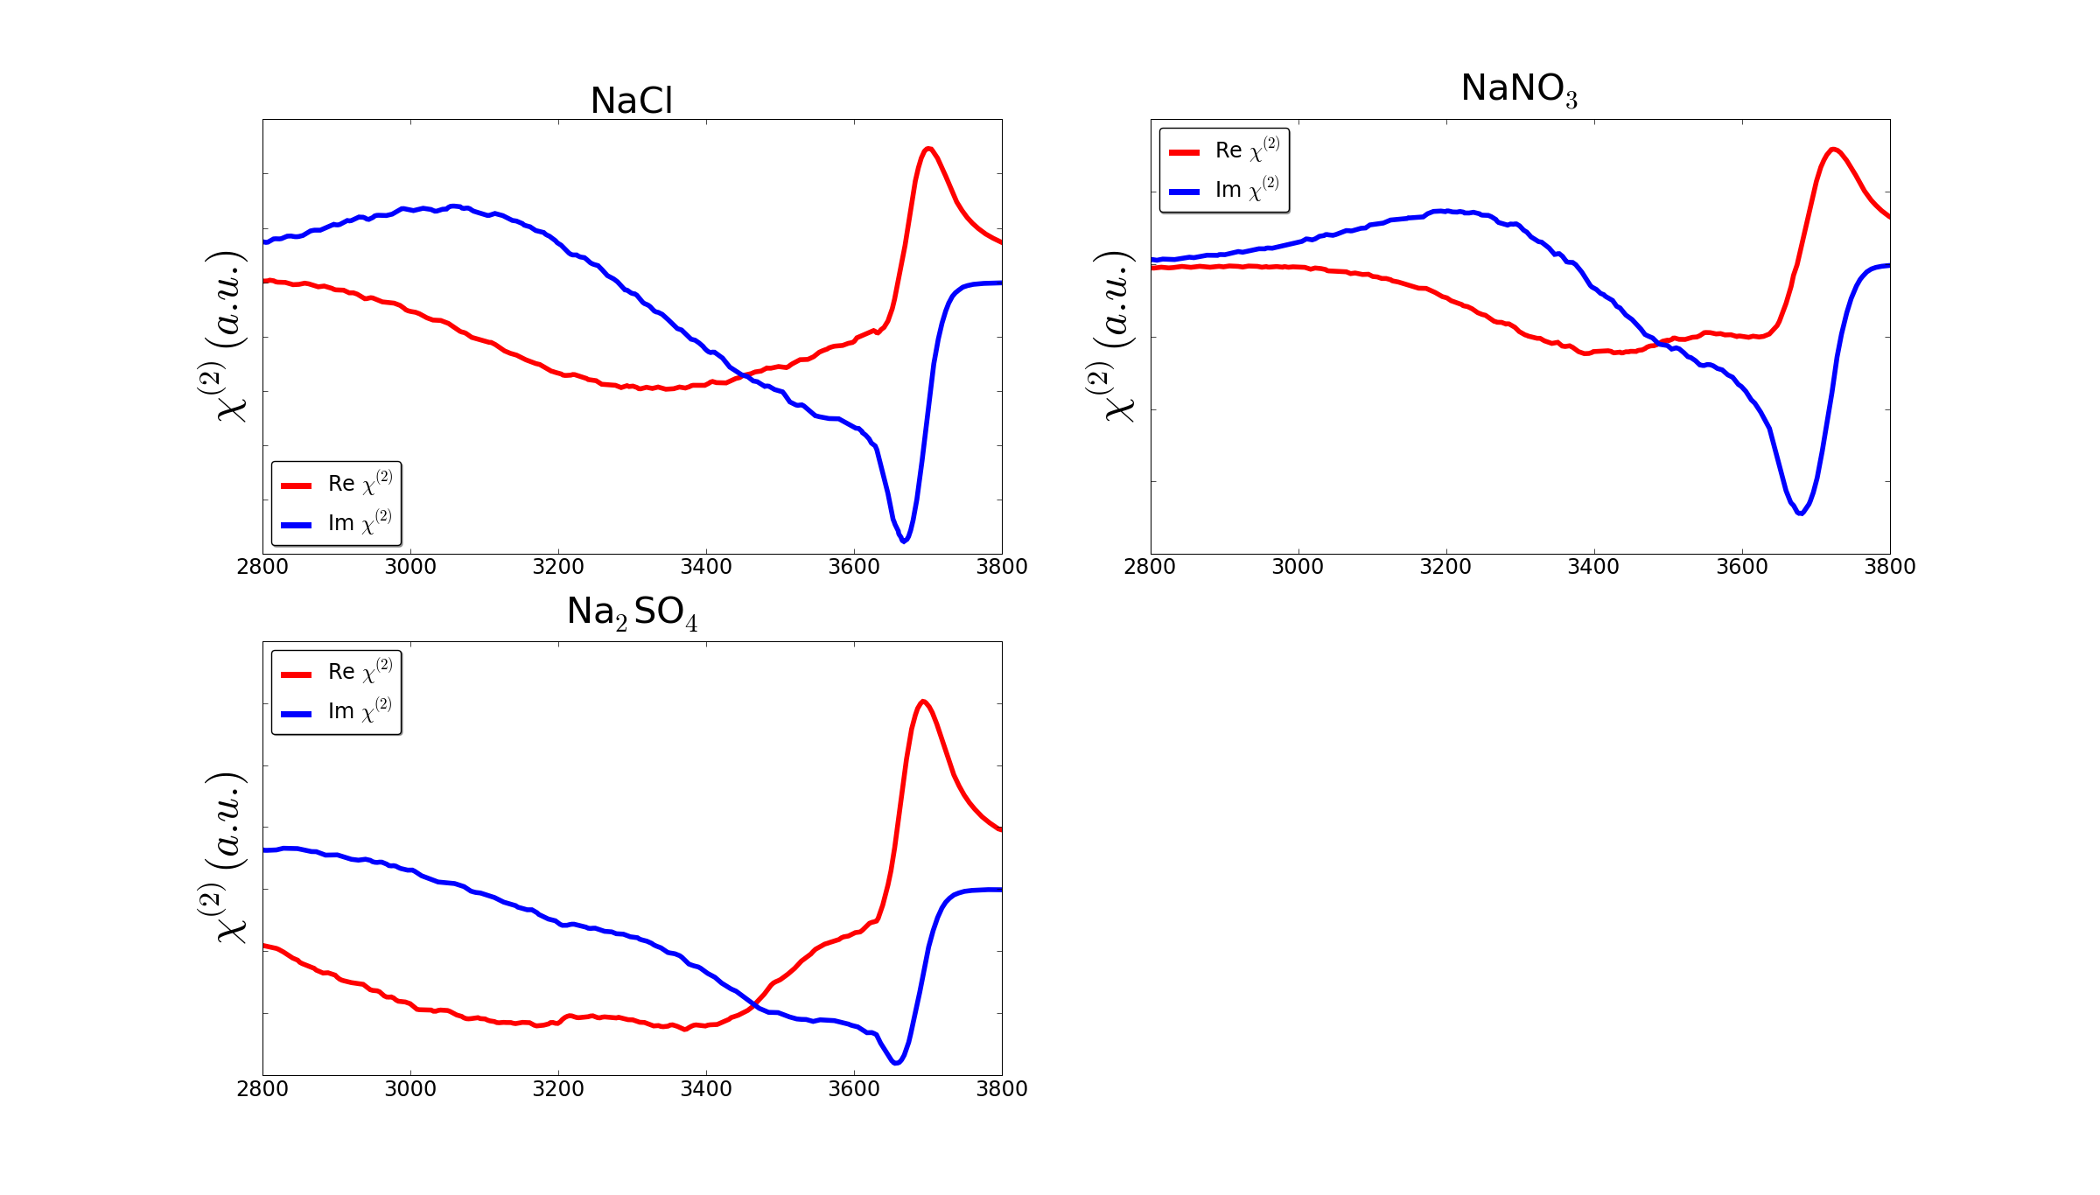
\includegraphics[scale=1.0]{images/chi2.png}
	\caption{Real and imaginary components of $\chi^{(2)}$ for the three aqueous salt solution interfaces.}
	\label{fig:chi2}
\end{center}
\end{figure}

\end{document}
